%----------------------------------------------------------------------------
\chapter{C-RAN koncepció}\label{sect:CranConcept}
A Telekommunikációs ipar az elmúlt években egy robbanásszerű fejlődésen ment keresztül az egyre növekvő forgalomigénynek köszönhetően.
Ez nem csak drasztikusan megnövelte a TCO-t (total cost of ownership, egy megközelítés mely segíti a vevőket és eladókat az egyes termékek árának meghatározására, az összes direkt és indirekt költséget beleszámolva), hanem egyre nehezebbé tette a fenntarthatóságát és az együttműködését a különböző hálózatoknak 2G, 3G, 4G és már beszélhetünk az 5G-ről is.\cite{RecentCRANProg}
A legújabb technológiák, mint a CoMP (Coordinated Multi-Point) ezeket a feladatokat igyekeznek maximálisan ellátni, ám a leghatékonyabb algoritmusaik (pl: JT-Joint Transmission) is kevesek, hogy a hagyományos X2 interface-el elérjék az LTE architektúra maximum teljesítőképességét, mely leginkább a nagy késési időknek és az alacsony sávszélességnek köszönhető. \cite{CoMP}
Végezetül a RAN (Radio Access Network)-ok nagy energia-fogyasztása is megemlíthető.
Ebben a fejezetben az architektúra főbb tulajdonságait és szerepét mutatjuk majd be.
%----------------------------------------------------------------------------
\section{Mi is az a C-RAN?}

\hspace{2mm}
\begin{wrapfigure}{r}{0.4\textwidth}
\captionsetup{format=plain}
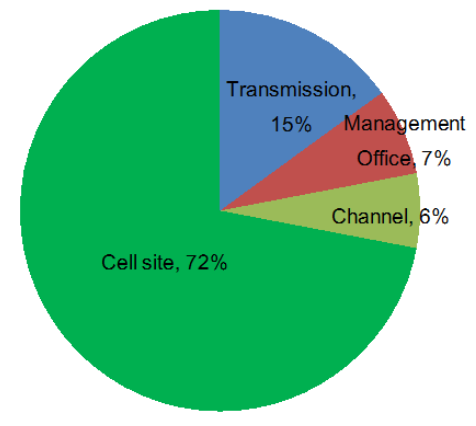
\includegraphics[width=0.4\textwidth, keepaspectratio]{figures/power_consumption.png}
\caption{A bázis állomások energia-fogyasztása a 72\%-a az össz energiafogyasztásnak. (China Mobile survey on commercial networks)}
\label{fig:power_consumption}
\vspace{-10pt}
\end{wrapfigure}
A C-RAN egy új RAN architektúra, melyet a China Mobile Research Institute mutattott be 2009-ben. Az akronímát, a tiszta, központosított, együttműködő felhőalapú RAN technológiára (Clean, centralized, collaborative, cloud) használják.\cite{RecentCRANProg}
A megalkotását a megnövekedett forgalomigények és a bázis állomások nagy energia-fogyasztása implikálta. Előbbi évről évre gyakorlatilag megkétszereződik, 2017-ben már a 20 ExaByte-ot is elérheti a Cisco adatai szerint, \figref{traffic}-es ábra. Utóbbiba pedig a China Mobile általános hálózati kutatása ad betekintést, a \figref{power_consumption}-as ábra alapján 72\%-át teszi ki az össz energia-fogyasztásnak.
A C-RAN rendszerek központosítják az alap feldolgozó erőforrásokat úgy, hogy azok egy egységes erőforráskészletet alkossanak, amiből dinamikusan az igényeknek megfelelően lehessen allokálni. Ezzel a technikával rengeteg előnyre tesz szert a hagyományos bázisállomás architektúrával szemben, mint például a megnövekedett erőforrás-használat, a kisebb energia-felhasználás, kisebb interferencia és a CoMP implementációk jobb támogatása. \cite{CoMP}
Fontos kiemelni azt, hogy a C-RAN nem csak egy könnyen alkalmazható technológia létező wireless hálózatok kiterjesztésére, hanem egy kulcsfontosságú elem az 5G-s hálózatok kialakítására.
Ez a technológia könnyen illeszthető megannyi 5G-s technológiához, mint a Large Scale Antenna Systems (LSAS)-hez vagy az ulta-sűrű full-duplex hálózatokhoz.\cite{TechOverview}

\begin{figure}[!ht]
\centering
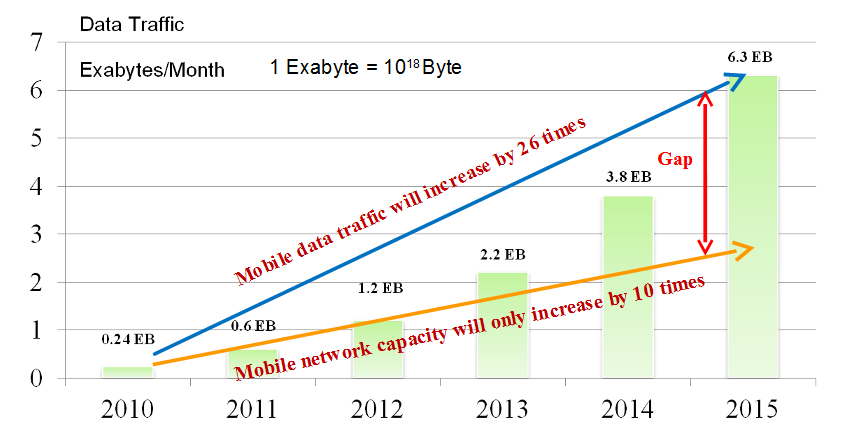
\includegraphics[width=\textwidth, keepaspectratio]{figures/traffic.png}
\caption{A mobil forgalomigények alakulása (Cisco VNI Mobile 2011)} 
\label{fig:traffic}
\end{figure} 

%----------------------------------------------------------------------------
\section{A C-RAN koncepciója}
\hspace{2mm} \indent Mint említettük, a C-RAN központosítja az alap feldolgozó erőforrásokat, hogy egy egységes erőforráskészletet alkossanak, amiből dinamikusan az igényeknek megfelelően lehet allokálni. Ennek alapkomponensei az elosztott BS-ek (base station-ok, bázis állomások). \cite{RecentCRANProg}
\begin{figure}[!ht]
\centering
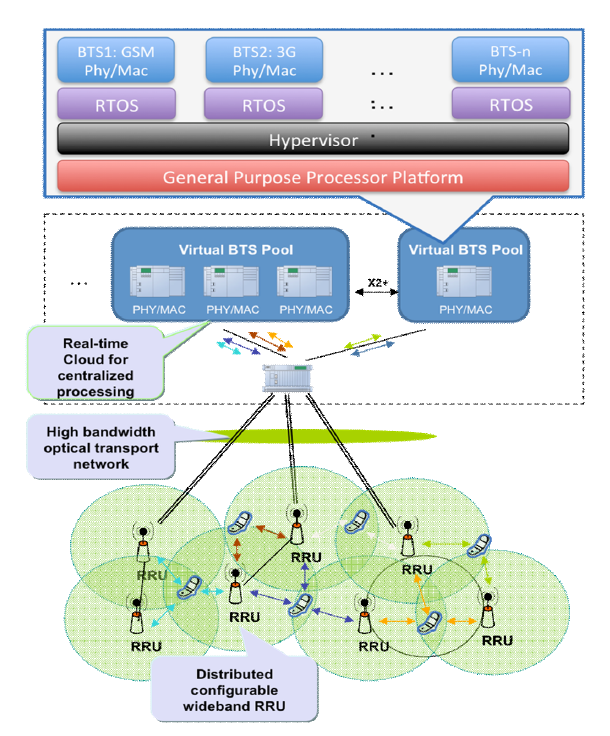
\includegraphics[width=\textwidth, keepaspectratio]{figures/cran_arch.png}
\caption{A C-RAN architektúra.\cite{RecentCRANProg}} 
\label{fig:cran_arch}
\end{figure} 

A \figref{cran_arch}-es ábrán szemléltetjük az architektúra három fő elemét.
\begin{itemize}
\item Base Band Unit (BBU) pool: Ez gyakorlatilag az erőforrás-készletünk, mely centralizáltan áll több időben változó mennyiségű soft BBU node-ból. A soft BBU nem más, mint egy hagyományos BBU aminek az erőforrásait és kapacitásit dinamikusan allokáljuk és újrakonfiguráljuk a valós-idejű követelményeknek megfelelve.
\item Remote Radio Unit networks: Ezek hagyomás RRU-k, a koncepció ezeken nem változtat, ők biztosítják az alap wireless lefedettséget
\item Transport networks: Ez az összekötő hálózat a BBU-k és az RRU-k között. Pontosítva egy készleten lévő BBU-t ez köt össze egy megadott RRU-val. Az alkalmazástól függően ez az összekötés teljesen más lehet, példákban láthatunk közvetlen vezetékes pl: sötétszálas kapcsolatot, mikrohullámú szállítást vagy üvegszálas kapcsolatot is.
\end{itemize}
%----------------------------------------------------------------------------
\section{Milyen előnyökkel jár a C-RAN?}
\hspace{2mm} \indent Elsőre csak egy központosított BBU hálózatnak tűnik a C-RAN architektúra, azonban a központosítás csak az első lépés a teljes kép megértéséhez. \cite{RecentCRANProg}
\begin{itemize}
\item BBU központosítás: az első alap feature a C-RAN hálózatokban.
\item Magas technológiai támogatás: A C-RAN pool-jához előkövetelmény egy minden-mindennel összekötött elválasztó-hálózat magas sávszélességgel és alacsony késési időkkel. Az elválasztó mechanizmus érzékeli az összeköttetéseket különböző számoló egységek között és megengedi a leghatékonyabb információáramlást közöttük. Ezek által a rendszer teljesítőképessége megnövekedhet.
\item Erőforrás virtualizáció, felhősítés: A hagyomásos rendszerek számítási kapacitásai limitálva vannak az egyes BBU-k erőforrásaiban és így az egyes node-ok az erőforrásaikat nem tudják megosztani egymással. Esetünkben viszont ezek a node-ok aggregálva vannak egy pool szinten és rugalmasan a kovetelmények alapján lehet őket allokálni.
\item "Soft" BBU: A hagyományos vezetéknélküli felszerelések a tulajdonosok saját platformjai lettek fejlesztve és kizárólag a saját "hard" fix tulajdonságokra tervezték őket, a legmagasabb adatforgalom elviselésére.
Azonban az erőforrások felhősítésével a BBU egy lágyabb "soft" erőforrás lett, melyet dinamikusan újra-konfigurálhatunk és igazíthatunk.
\item A szolgáltatások telepítésének elősegítése a végpontokon: A C-RAN hálózatok nagyobb területket fednek le és több felhasználót látnak el, mint a már megszokott bázis állomások. Ezáltal az egyes szolgáltatások mozgatása, vagy új szolgáltatások telepítése a RAN oldalon egyszerűbbé vált, így egyrészt fokozható a User Experience (felhasználói élmény), másrészről kevésbé terheli a gerinchálózatot.
\end{itemize}
%----------------------------------------------------------------------------
\section{C-RAN Kihívásai}
\hspace{2mm}  \indent Az első probléma, amibe ütközünk az összeköttetések, optikai kábelek mértéktelen szükségessége, melyből mint erőforrás nem áll annyi rendelkezésünkre. A front-haul-t úgy definiálták, mint a BBU-t és az RRU-t összekötő hálózat, a tipikus front-haul protokollok a Common Public Radio Interface (CPRI) és az Open Base-station Architecture Initiative (OBSAI). Az üvegszálhasználat csökkentésére rengeteg kompressziós technikát kitaláltak, de megemlíthetjük az SFDB-t (Single Fiber Bi-direction) is mely megengedi az egy szálon történő szimultán UL és DL, fel és letöltést. Egy másik ötlet a WDM (Wavelength-division multiplexing), mely a hullámfelosztással rengeteg vivőjelet enged meg a szál felosztásával, bár ezzel a zajt és a késések is növelve.
\vspace{-20pt}
\begin{wrapfigure}{r}{0.5\textwidth}
\captionsetup{format=plain}
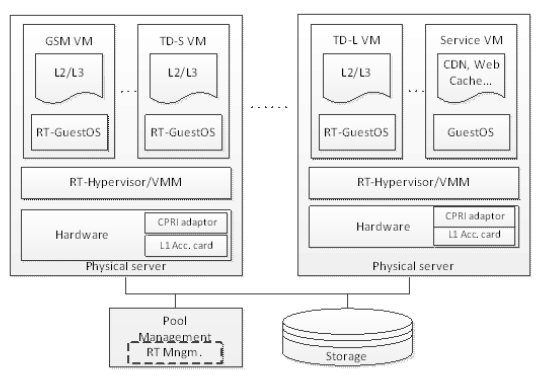
\includegraphics[width=0.5\textwidth, keepaspectratio]{figures/virtualisation.png}
\caption{RAN virtualizáció}
\label{fig:virtualisation}
\vspace{-20pt}
\end{wrapfigure}

\indent A második nagy kihívás az erőforrások felhőszintű használata, virtualizálása. Mivel eddig mindenki a saját magának megfelelő BBU-t használta, így ki kell fejleszteni egy új BBU entitást, mely mindenkinek kedvező és azon a virtualizációs technológiákon alapul, amelyek a modern Adatközpontokban már jelen vannak. Egy egész jól illeszkedő megoldás lehet a Network Function Virtualization (NFC), ami rengeteg hálózat típust konszolidál ipari nagykapacitású szerverekbe, switchekbe és kapacitásba, amik már elhelyezkedhetnek adatközpontokban, hálózati egységekben vagy akár a usereknél maguknál. \cite{NFV}
A virtualizáció megvalósítását mutatja a \figref{virtualisation}-es ábra. A bázis erőforrás pool több standard IT szerverből áll, és minden szerverhez tartozik egy dedikált hardver gyorsító, hogy a számolásigényes feladatokat a fizikai réteg el tudja látni. Ezeknek a gyorsítóknak meg kell felelniük a valósidejű vezetéknélküli jelfeldolgozási követelményeknek, így az L2/L3-as funkciók egy-egy virtuális gépen futnak, virtuális környezetben. A további felhasználói applikációk, mint a Web-Cache ugyancsak futhatnak ebben a virtuális környezetben. Ezek elsőre könnyen megérthetőnek tűnnek, azonban a real-time feldolgozásnak nagyon szigorú követelményei vannak, így nagyon nagy feladatról beszélünk.\cite{RecentCRANProg}

\hspace{2mm}
\begin{figure}[!ht]
\centering
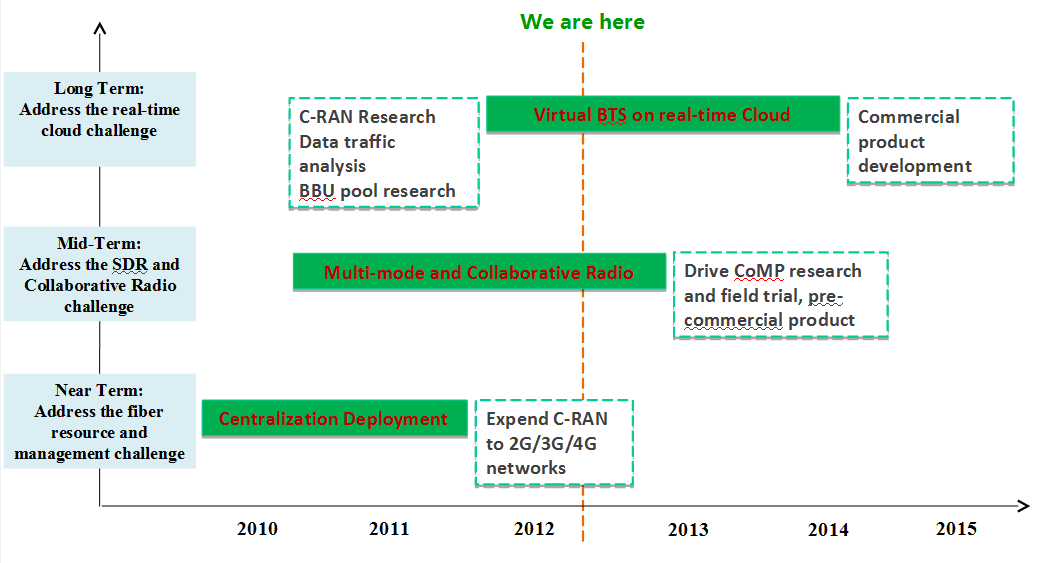
\includegraphics[width=\textwidth, keepaspectratio]{figures/timeline.png}
\caption{A C-RAN legfontosabb fejlődési lépései} 
\label{fig:timeline}
\end{figure} 

\indent A C-RAN-nak képesnek kell lennie minden a modern hálózatok által elfogadott feladatok ellátására, ezeket majd az implementációnál is figyelembe kell vennünk, így érdemes végignézni a C-RAN fejlődéstörténetét a \figref{timeline}-es ábra segítségével.
\begin{itemize}
\item Valamilyen úton-módon a régebbi rendszerekhez kapcsolódnia kell, amellyel végső soron elérhető lenne a teljes hálózat egyszerűsítése az egységes hálózati architektúrának köszönhetően.
\item Képes kell legyen elválasztani a szabályozási és felhasználói szintet, hogy rugalmasan méretezhető teljesítményt biztosítson a RAN különböző funkciói számára.
\item Számos fejlesztési lehetőséggel kell rendelkeznie a hálózati struktúra területén, (pl. széleskörű transzport hálózati megoldások, bázisállomás konfigurációk és felhasználói alkalmazások)
\end{itemize}
Ha az utolsó implementációs pontot is sikerül meglépnünk, akkor elkezdődhet a tömegszerű felhasználás.